\section{Introduction}
\label{sec-intro}

In recent years, visual question answering (\vqa) has received significant attention~\cite{malinowski2015ask,ren2015image,gao2015you} as it involves multi-disciplinary research, \eg natural language understanding, visual information retrieving and multi-modal reasoning. The task of \vqa is to find an answer to a question $\nlq$ based on the content of an image. There are a variety of applications of \vqa, \eg surveillance video understanding, visual commentator robot, \etc. Solving \vqa problems usually requires high level reasoning from the content of an image.

\begin{figure}[tb]
\centering
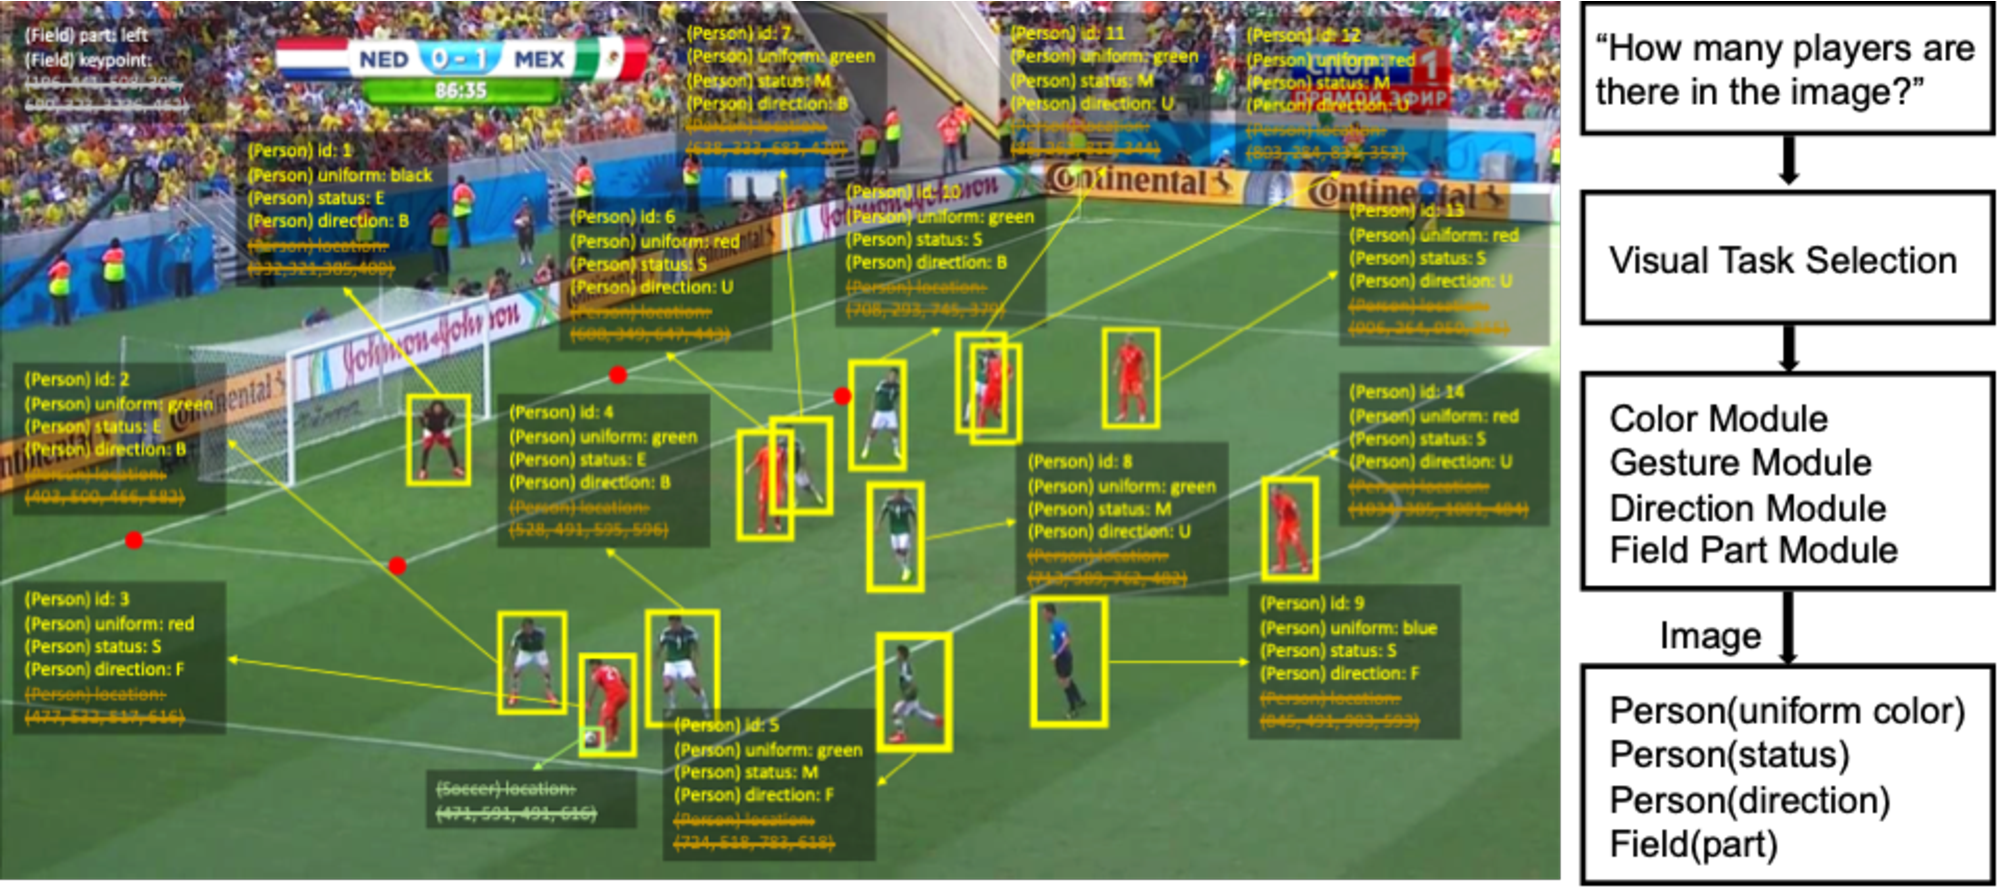
\includegraphics[width=\columnwidth]{motivation.eps}
\caption{The image is about soccer match, where each person object is associated with attributes: id, uniform color, status (\underline{S}tanding, \underline{M}oving, \underline{E}xpansion), direction (\underline{B}acking, \underline{F}acing, \underline{N/A}), as well as location, and the soccer object is attributed with location. %Part (b) shows a part of corresponding entity-attribute graph. Part (c) exhibits a $\nlq$ and its corresponding query graph $Q$. 
}
\vspace{-4ex}
\label{fig:example}
\end{figure}


\begin{example}
Figure~\ref{fig:example} depicts an image about a soccer match, where two teams are distinguished by red and green uniforms, and each object is associated with a set of attributes. A typical query may ask ``How many players are there in the image?''. Though simple, it is a challenging task to efficiently answer the query, since (1) it is often very inefficient to detect all the objects in the given image, following traditional way, while only query related objects are in demand; (2) one not only needs to identify all the {\em person} objects, but also have to infer their hidden attribute ``role'', which is often ambitious. 

Motivated by these, one may analyze questions first and detects only those objects as well as their attributes that are in connection with questions, then infer missing values of hidden attributes, and answer questions. In this way, not only query accuracy but also query efficiency are expected to be guaranteed.  
\end{example}


This example suggests that we leverage adaptive query understanding and reasoning to address the \vqa problem. While to do this, two critical questions have to be answered. (1) How to understand queries and carry query-related visual tasks? (2) How to infer crucial information to assist query answering?  


\vspace{2ex}
\stitle{Contributions.} In contrast to a majority of deep learning based \vqa techniques, which not only overlooks correlation between queries and images, but also lacks of necessary reasoning, we propose a novel technique that integrates adaptive query understanding and reasoning.  The main contributions of the paper are as follow.  

(1) We model images and queries as graphs, and propose to answer visual queries with graph matching. This new representation and answering scheme constitute the base of our techniques.  

(2) We introduce a method to guide visual tasks based on reinforcement learning. That is, given an image and a question, our method can identify a set of visual tasks that are question related, and direct subsequent visual processing in a more efficient manner. 

(3) We propose approaches to answering visual queries based on reasoning and graph matching. More specifically, we first transform a given image into an entity-attribute graph; we then develop method to infer missing value for question answering; %As verified in our empirical studies, the classifier is very effective, with accuracy reaching X\%. 
we finally show how to answer queries with graph matching. %To this end, we first transform a natural language query into a pattern query, and then employ matching technique to find answers. 

4) We conduct extensive experimental studies to verify the performance of our method. We find that X, Y, and Z. 